%\title{BIO 360 Evolution Review Paper}
\documentclass[12pt]{article}
\usepackage[utf8]{inputenc}
\usepackage{ifpdf}
\usepackage{mla}
\usepackage{sidecap}
\usepackage{setspace}
\usepackage{subcaption}
\usepackage{csquotes}
\usepackage{mathptmx}

\usepackage{siunitx}
\DeclareSIUnit\molar{\mole\per\cubic\deci\metre}
\DeclareSIUnit\Molar{\textsc{m}}

\usepackage{titlesec}
\titleformat{\section}
  {\normalfont\large\raggedright}{\thesection.}{1em}{}
\titlespacing\section{0pt}{12pt plus 4pt minus 2pt}{0pt plus 2pt minus 2pt}
\titleformat{\subsection}
  {\normalfont\large\raggedright}{\thesubsection.}{0.75em}{}
\titlespacing\section{0pt}{12pt plus 4pt minus 2pt}{0pt plus 2pt minus 2pt}

\usepackage{etoolbox}
\appto\displayquote{\singlespacing}

\setlength{\parindent}{0.25cm}
\setlength{\parskip}{0em}

\makeatletter
\title{The Lenski Long Term Evolution Experiment}\let\Title\@title
\author{Matthew Moreno}
\makeatother

% keep all footnotes on the same page
\interfootnotelinepenalty=10000

\linespread{1.25}

\begin{document}

\begin{mla}{Matthew}{Moreno}{Professor Vanessa Koelling}{BIOL 360}{May 12, 2017}{{\large \Title}\vspace{-1ex}}

\section{Introduction} \label{sec:introduction}

As popularly conceived, evolutionary biology stands somewhat apart from many other branches of science.
Significant effort among evolutionary biologists focus on developing an understanding for how contemporary diversity of life came to be.
The historical contingency of the subject matter makes some questions addressed by evolutionary biology very difficult to explore through reproducible experimentation to attempt to falsify currently held hypotheses, the primary tool of scientific inquiry \cite{Smith2016ExplanationsBiology}.
For example, it would be difficult to test, in the traditional experimental fashion, the hypothesis that hairlessness evolved in hominid precursors due to natural selection for its capability to facilitate evaporative cooling.
That is, it would be near impossible to conduct alternate trials under different conditions to observe if the hypothesis is sufficient to explain the outcome.
This is not to say that empirical evidence does not exist for these claims: it does, and in overwhelming proportions.
In fact, in several cases evolutionary theory predicted yet-undiscovered empirical evidence, such as the amphibian-fish intermediate fossil \textit{Tiktaalik roseae} \cite{Daeschler2006APlan}.

Nonetheless, repeatable experiments are a desirable piece of the scientific puzzle of evolutionary biology.
Post hoc explanations for a phenomenon suffer inherent bias.
Fit between hypothesis and observation in traditional experimental work is interpreted as strong evidence for the validity of the explanation.
However, fit of the hypothesis and observation cannot be interpreted as strong evidence for the validity of the hypothesis due to the ``powerful psychological mechanism of hindsight bias'' \cite{Smith2016ExplanationsBiology}.
Essentially, ex post facto explanations always match the evidence they describe because they were created exactly to do so.
From this well is drawn the accusation of the ``just-so story'' commonly leveled against aspects of evolutionary biology \cite{Smith2016ExplanationsBiology}

Repeatable experiments have been employed to great effect in other scientific endeavors to understand natural history, like geology and cosmology.
This work has been present throughout the history of evolutionary biology; for example, the development of modern genetics has provided a firm underpinning for the notion of heritable variation necessary to evolutionary theory.
It was through repeatable experiments, such as Mendel's work with peas or the Hershey-Chase experiments, through which this aspect of our understanding of evolution was established \cite{Griffiths2015IntroductionAnalysis}.
Experimental work continues to serve as a foundation of modern evolutionary biology.
The work of the Bradshaw group exemplifies experimental work performed in the field.
This group uses experimental techniques to develop a detailed and concrete account of aspects of the evolutionary story, establishing, for example, how specific genetic changes in the California Monkeyflower manifest in phenotypic changes that, in turn, observably affect pollinator behavior in such a way as to promote reproductive isolation \cite{Byers2014FloralMimulus}.
Such experimental work in evolutionary biology tends to focus in on a specific component of the evolutionary process such as the genetic basis of heritable phenotypic variation or the manner in which phenotypic traits interact with the environment in regards to selection.
At most, experimental evolution tracks the evolutionary changes in response to experimental treatments over tens or hundreds of generations.
Famous examples of such efforts include long-term evolutionary experiments with the common fruit fly \textit{Drosophila melanogaster} \cite{Rose1984ArtificialMelanogaster}, unicellular yeast \textit{Saccharomyces cerevisiae} \cite{Ratcliff2012ExperimentalMulticellularity.}, and experiments observing \textit{E. coli} over hundreds of generations \cite{ATWOOD1951PeriodicColi.}.
Performing experiments to delve into evolution on a larger scale is difficult, expensive, and, critically, time-consuming.
Such experiments are inherently rate-limited by the generation-time of their experimental subjects.

It is into this relatively underexploited and important scientific terrain --- evolutionary biology experiments that unfold over vast stretches of generation on generation unfolding --- that the Lenski laboratory launched its Long Term Evolution Experiment (LTEE) in the year 1988 \cite{Lenski2017TheSite}. 
The aim of this work was to better understand how natural selection, historical constraint, and serendipity contribute to the adaptation of species and divergence between species observed in biology.
It was specifically hoped to observe long-term trajectories of mean fitness and genetic variation in fitness within and between groups sharing a common ancestor evolving in parallel \cite{Lenski1991Long-TermGenerations}.
In order to assess these questions in a timely and economical fashion, the experiment was carried out with a bacterial strain, \textit{E. coli}.
As of March of 2017, the Lenski experiment had surpassed 67,000 successive generations of experimental \textit{E. coli} evolution.
The project has generated rich theoretical insight into the questions it was conceived to address.
Moreover, it has generated a rich biological library of \textit{E. coli} that were suspended at regular intervals throughout the evolutionary process.
The biological materials generated by the LTEE have been leveraged by other researchers to investigate questions ranging from DNA supercoiling \cite{Crozat2010ParallelColi} to population divergence resulting in the occupation of a new ecological niche \cite{Plucain2014EpistasisColi}.
The LTEE has attracted a fair amount attention, both from scholarly and popular audiences \cite{Dawkins2009TheEvolution, Zimmer2009MicrocosmLife, Zimmer2011TortoiseFlask, Lenski2016EvolutionaryLenski}.
This notoriety stems, in part, from the feats of endurance and tireless exacting execution that were required to successfully sustain the LTEE over several decades.
The project is also recognized for the scientific value that the experiment has yielded, and continues to yield, with the elapse of generation upon generation of laboratory-reared \textit{E. coli}.

\section{Experiment}

\begin{SCfigure}
  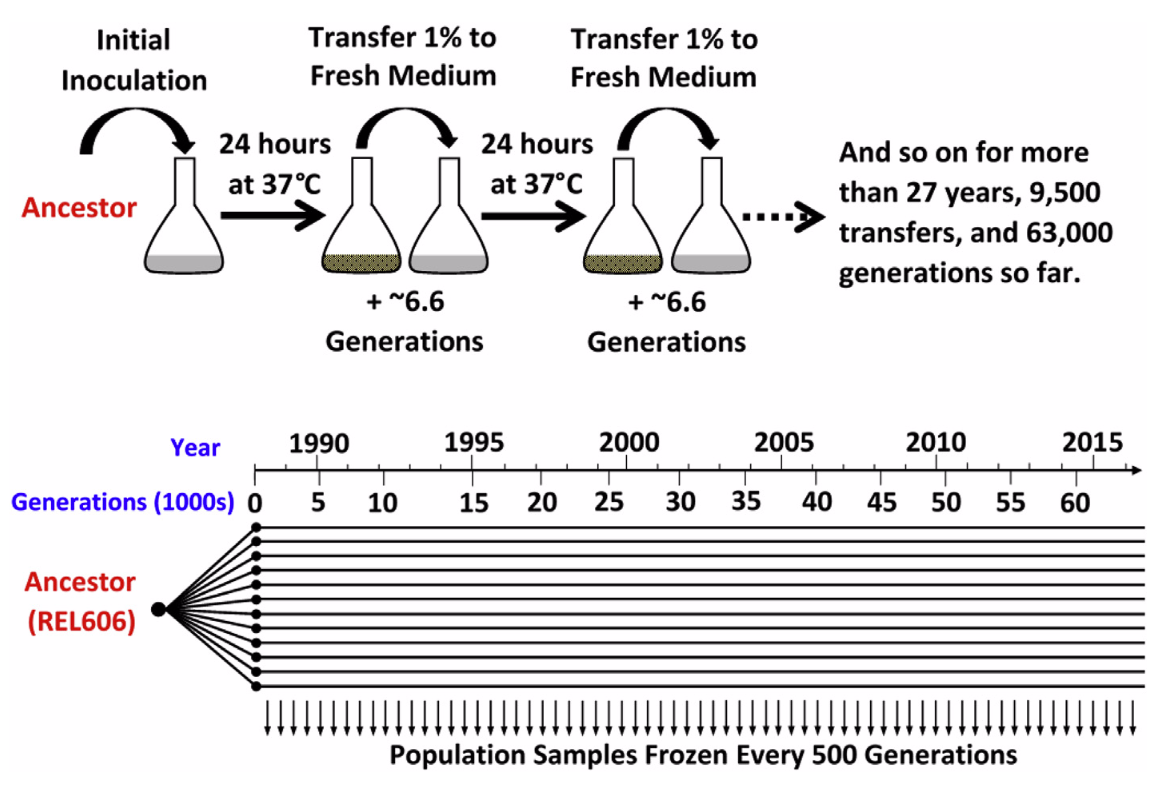
\includegraphics[width=0.7\textwidth]{img/ltee_schematic}
  %\captionsetup{singlelinecheck=off,justification=raggedright}
  \hspace{2ex}
  \caption[Overview of the Lenski \textit{E. coli} Long-Term Evolution Experiment]{In the LTEE, twelve \textit{E coli.} strains are propagated through daily serial transfers. Every 24 hours, during which time approximately 6.6 generations elapse, 1\% of the population is extracted and placed in fresh growth medium \cite[Figure 1]{Blount2016AContingency}.}
  \label{fig:ltee_schematic}
\end{SCfigure}

As depicted in Figure \ref{fig:ltee_schematic}, at its core the Lenski LTEE follows the parallel evolution of a dozen \textit{E. coli} lineages.
These lineages are maintained in separate liquid growth mediums. 
Daily transfers install a small fraction of the existing population in a fresh medium \cite{Blount2016AContingency}.
Every 500 generations, samples from the remaining population after transfer of \textit{E. coli} to fresh media are frozen away at \SI{-80}{\celsius} in glycerol \cite{Lenski2017TheSite}.
These biological archives allow for later detailed analysis of the genetic and phenotypic changes each lineage experienced over the course of the experiment \cite{Blount2012GenomicPopulation} and for critical evolutionary periods to be replayed in replicate \cite{Turner2015ReplayingPopulation}.

The B strain of \textit{E. coli} employed in the LTEE was selected for traits that make accounting for genetic material straightforward. 
The \textit{E. coli} strain chosen propagates exclusively through strict clonal descent --- the strain does not harbor plasmids or functional bacteriophages or reproduce sexually \cite{Lenski1991Long-TermGenerations}.
Hence, novel genetic traits can be attributed with high confidence to \textit{de novo} mutation events that occurred within the course of the experiment.
The strain also exhibits the handy characteristics of short generation time (approximately six generations per day), ability to be suspended indefinitely in glycerol at \SI{-80}{\celsius} and subsequently reanimated, and well-developed biological and procedural characterization due to its common use in laboratory experiments \cite{Lenski2017TheSite,Lenski1991Long-TermGenerations}.
Additionally, the strain selected was specifically sensitive to bacteriophage T5 and resistant to bacteriophage T6.
This property, which differentiates the B strain of \textit{E. coli} from other \textit{E. coli} and other bacteria, allows the LTEE lineages to be readily checked for cross-contamination \cite{Lenski2017TheSite}.

In the Lenski LTEE, E coli. are cultured in the Davis minimal broth, also known as DM25. 
Thiamine hydrochloride and glucose are added to the broth at 
concentrations of \SI{2e-6}{\gram\per\liter} and \SI{2.5e-2}{\gram\per\liter}, respectively \cite{Lenski1991Long-TermGenerations}. 
The glucose concentration was set so that the supply of this nutrient would be quickly exhausted by the growth of \textit{E. coli}.
Thus, the populations cycle daily between satiety and resource exhaustion \cite{Blount2016AContingency}.
Citrate, which turned out to represent a potential alternate food source for \textit{E. coli}, is present in the DM25 broth at a significant concentration of \SI{1700}{\micro\Molar}.
This amounts to more than ten times the concentration of glucose.
At the outset of the experiment, citrate was included simply  to conform to the established recipe for the DM25 broth \cite{Blount2016AContingency}.
The \textit{E. coli} B strain chosen by Lenski to found the LTEE's dozen lineages is incapable of aerobically metabolizing citrate, although \textit{E. coli} can ferment the compound in an Oxygen-poor environment \cite{Blount2016AContingency}.
This inability of \textit{E. coli} to metabolize citrate aerobically stems from the regulation of the citrate transporter CItT, which is exclusively expressed in anaerobic environments \cite{Pos1998TheChloroplasts}.

The B strain of \textit{E. coli} selected by Lenski et al. also did not exhibit an ability to metabolize the sugar L-arabinose.
At the outset of the experiment, a large number of cells of the strain screened for the ability to synthesize L-arabinose.
A colony of such cells was isolated.
The ability to metabolize L-arabinose proves a useful indicator.
Colonies capable and incapable of L-arabionse metabolization can be readily distinguished on tetrazolium arabinose indicator plates, with the former taking on a white color in contrast to the red color taken on by the latter.
Strains of \textit{E. coli} capable and incapable of metabolizing L-arabinose are described as Ara$^+$ and Ara$^-$, respectively \cite{Lenski1991Long-TermGenerations}
The original B strain of \textit{E. coli} acquired by Lenski et al. and the Ara$^+$ variant isolated from the original strain were specifically deemed REL607 and REL606, respectively \cite{Lenski2017TheSite}.
Although the Ara$^+$ strain uniquely exhibits the ability to metabolize L-arabinose sugar, the two strains were demonstrated to exhibit relative fitness of 1.00 +- 0.01 (95\% confidence interval) under the LTEE experimental conditions \cite{Lenski1988ExperimentalT4}.

Of the dozen lineages in the LTEE, six were founded from the REL606 strain and six were founded from the REL607 strain.
Maintaining both Ara$^+$ and Ara$^-$ lineages provides a methodological avenue for the assessment of fitness.
The fitnesses of two populations, one Ara$^+$ and the other Ara$^-$, relative to one another are assessed by:
\begin{enumerate}
\item growing each population separately in a liquid culture for a day,
\item mixing equal parts volume of both populations together in a fresh liquid medium and incubating for another day,
\item plating out the dual-population mixture on tetrazolium arabinose indicator plates, then
\item counting out colonies from each population based on the alternate colorations.
\end{enumerate} 
In the LTEE, three different types of fitness assessments were performed by placing clones from each of the evolved lineages in competition against baseline clones of the opposite Ara marker type and against clones from an alternate lineage within the same generational cohort of the opposite Ara marker type
\cite{Lenski1991Long-TermGenerations}.
In the course of the experiment, the Ara$^+$ and Ara$^-$ markers also provided a useful mechanism to detect inadvertent contamination.
Daily transfers strictly alternate between Ara$^+$ and Ara$^-$ strains \cite{Lenski2017TheSite}.
Periodic checks are made for cross-contamination between LTEE lineages using tetrazolium arabinose indicator plates \cite{Lenski1991Long-TermGenerations}.
At each daily transfer, backup copies of the lineage from the previous day are kept in the refrigerator to allow ready recovery in the event of a mishap \cite{Lenski2017TheSite}.




\section{Results} \label{sec:results}

As was discussed in Section \ref{sec:introduction}, the Long Term Evolution Experiment has allowed researchers to address a broad set of questions of interest to evolutionary biology.
We will briefly discuss just three here.
First, Section \ref{sec:potentiation} discusses the question the experiment originally set out to investigate: the role of historical contingency in evolution.
The evolution in one of the replicate lineages of a capacity to metabolize citrate aerobically, an unexpected phenomenon, has provided great insight into this domain. 
Two other unexpected phenomenon, the evolution of traits that significantly altered mutation rates and the emergence and long-time coexistence of distinct sub-lineages in one of the LTEE lineages, have shed light on questions of evolvability and niche specialization. 
These topics are discussed in Sections \ref{sec:evolvability} and \ref{sec:niche} respectively.

\subsection{Potentiation} \label{sec:potentiation}

To the surprise, and initial suspicion, of LTEE researchers, in 2003 --- when approximately 33,000 generations of experimental evolution had elapsed --- the lineage Ara-3 developed the capacity to aerobically metabolize citrate.
As this change significantly expanded the food supply available to the \textit{E. coli} population, the change manifested as significantly cloudier cultures.
Experiments plating these cells on media with citrate as the exclusive food source confirmed that, indeed, a Cit$^+$ phenotype had emerged.
Further studies confirmed that cells exhibiting the Cit$^+$ phenotype were descended from the Ara-3 population and were not an artifact of contamination \cite{Blount2008HistoricalColi.}.
The Cit$^+$ phenotype was later revealed to stem from duplication of the gene encoding the CItT transporter under a new promoter, enabling its expression, and therefore the import of citrate, under aerobic conditions \cite{Blount2012GenomicPopulation}.
This late emergence of the Cit$^+$ phenotype in only one replicate lineage, despite the availability of citrate to all twelve LTEE lineages throughout the entire experiment, left researchers curious about the evolutionary path the Ara-3 lineage had traced.

It was hypothesized that so-called potentiating mutations, genetic changes with neutral or unrelated phenotypic consequences that are nonetheless necessary to observe mutations that enable the Cit$^+$ phenotype, had taken place in the Ara-3 lineage
\cite{Blount2016AContingency}.
Using samples suspended at various points in the history of the Ara-3 lineage, experiments plating out trillions of cells to screen for spontaneous mutations enabling Cit$^+$ as well as more extended experimental replays of evolution both support this hypothesis \cite{Blount2008HistoricalColi.}.
The Cit$^+$ phenotype was never observed among offspring from baseline members of the Ara-3 lineage. 
Among  members  of the Ara-3 population several generations before Cit$^+$ was observed to emerge, the Cit$^+$ phenotype was observed to occur  more frequently from members of the specific sublineage from which Cit$^+$ originally emerged than from members of other  contemporary clades.
This led researchers to suspect that at least two potentiating mutations had taken place \cite{Blount2012GenomicPopulation}.
A mutation to the \textit{gltA} gene, which is known to encode citrate synthase, is thought to have served as a potentiating mutation.
This muation improved metabolic function in the presence of acetate (which was generated by cells from a different sublineage).
Coincidentally, it also enabled metabolic benefit to be derived from promoter reassignment of the gene encoding CItT \cite{Blount2016AContingency}.
The identification of other potentiating mutations remains an open question.

\subsection{Evolvability} \label{sec:evolvability}
A significant increase in the rate of mutation occurrence --- a full order of magnitude greater than the baseline REL606 and REL607 populations --- was observed among three LTEE lineages at generation 10,000, Ara$^-2$, Ara$^-4$, and Ara$^+3$  \cite{Sniegowski1997EvolutionColi}.
Injection of plasmids containing wild type copies of seven known mutator locis into cells from these strains were able to rescue mutation rate to its previous lower state.
In such a manner, the high rate of mutation occurrence was ascertained to stem from defects in the methyl-directed mismatch repair pathway in these lines \cite{Sniegowski1997EvolutionColi}.
It was hypothesized that mutator alleles had ``hitch-hiked'' to ubiquity due to their association with unrelated mutations that conferred a significant fitness benefit.

Subsequently, a hypermutator phenotype stemming from a frame-shift mutation to the gene \textit{mutT} was observed to emerge in the Ara–1 population of the LTEE around generation 20,000.
Over the course of the next several thousand generations, alterations to the gene \textit{mutY}, which somewhat reduced the high mutation rate introduced by mutation to \textit{mutT} were observed in two sub-lineages of the Ara-1 population.
Researchers posit that this case might follow a pattern where higher mutation rates are favored by natural selection for a time but are later replaced by lower mutation rates as populations become well adapted to their environments \cite{Wielgoss2013MutationLoad.}.

\subsection{Niche Specialization} \label{sec:niche}
Around generation 6,000, a distinct pair of phenotypes began to be observed among colonies plated up from the LTEE population Ara-2. 
Some cells quickly formed large colonies while others formed only small colonies, even after the passage of an extended period of time.
The former were deemed L cells and the latter, S cells.
Phylogenetic analysis revealed that these two groups were monophyletic.
That is, a divergent pair of phenotypically differentiated but coexisting lineages were observed.
These lineages persisted together for 12,000 generations \cite{Rozen2005Long-termPolymorphism}.

The long duration in which these alternate phenotypes persisted led researchers to hypothesize that frequency-dependent selection was at play.
Indeed, it was shown that although L grows faster, S persists better after exhaustion of the daily glucose supply in the media.
Additionally, it was discovered that the growth of S is promoted by a metabolite excreted by L \cite{Rozen2005Long-termPolymorphism}.
Given the extreme simplicity of the experimental environment that the LTEE populations inhabit, the long-term coexistence of alternate survival strategies --- an apparent emergence of niches --- is a surprising result.

\section{Conclusion} \label{sec:conclusion}

The Lenski Long Term Evolution Experiment exquisitely demonstrates the unique opportunities for insight afforded by experimental evolution.
Studying the process of evolution in the laboratory allows for unparalleled repeatability, control over experimental conditions, and an ability for holistic measurement and observation.
As discussed in the preceding sections, these factors have enabled detailed study of specific evolutionary events that took place over the course of the LTEE, which has shed light on big questions, such as the evolutionary roles of historical contingency and mutational modulators.
As detailed in Section \ref{sec:introduction}, despite its notoriety the LTEE is by no means unique in its pursuit of experimental evolution.
In 2010, the Lenski laboratory became affiliated with a larger coallition to to study ``evolution in action,'' the NSF-funded BEACON Center \cite{Lenski2017TheSite}.
In addition to \textit{in vivo} work such as the Lenski LTEE, the BEACON Center was founded to support experimental evolution work both \textit{in silico}.
Excitingly, hybrid \textit{in silico}-\textit{in vivo} research, such as work to understand the relationship between population structure and evolutionary innovation, trialled in digital simulation then confirmed in the petri dish \cite{Nahum2015ABacteria.}, has also begun to emerge from the Center. 
Given the unique perspective provided by experimental evolution, the continuing LTEE and other experimental evolution projects that have begun to flourish at the BEACON center promise to yield exciting evolutionary insight far into the future.


\newpage
\bibliography{Mendeley}
\bibliographystyle{apalike}


\end{mla}

\end{document}

